\chapter{The Compact Muon Solenoid Experiment}
\label{chap:I-3-cms}

	The Compact Muon Solenoid (CMS) \cite{1748-0221-3-08-S08004} is a multi-purpose particle detectors recording the collisions provided by the LHC. It was, along with ATLAS, the first experiment officially approved for the LHC by the CERN research board in January 1997 after a long evalution process of the letter of intent published four years earlier by the two collaboration. The construction of the detector started in 2005, after the excavation works of the cavern finished, and spanned until 2008. Since then, CMS has been proficiently recording and analyzing data, and announced on July 4th 2012 the discovery of the Brout-Englert-Higgs boson, one of the most significant results of the collaboraton.

  \section{Overview}

    At nominal energy and luminosity, the LHC produces around 20 proton-proton collisions per BX which results in around 1000 particles in the final state. In order to identify physical processes with great precission, CMS has to ensure good identification and reconstruction of the particles. To this end, the detector was built around four requirements:
    \begin{itemize}
      \item Good muon identification and momentum resolution over a wide range of momenta and angles, good dimuon mass resolution ($ \approx $ 1\% at 100 GeV), and the ability to determine unambiguously the charge of muons with p < 1 TeV;
      \item Good charged-particle momentum resolution and reconstruction efficiency in the inner tracker. Efficient triggering and offline tagging of $ \tau $'s and b-jets, requiring pixel detectors close to the interaction region;
      \item Good electromagnetic energy resolution, good diphoton and dielectron mass resolution ($ \approx $ 1\% at 100 GeV), wide geometric coverage, $ \pi^0 $ rejection, and efficient photon and lepton isolation at high luminosities;
      \item Good missing-transverse-energy and dijet-mass resolution, requiring hadron calorimeters with a large hermetic geometric coverage and with fine lateral segmentation. \\
    \end{itemize}

    \begin{figure}[h!]
      \centering
      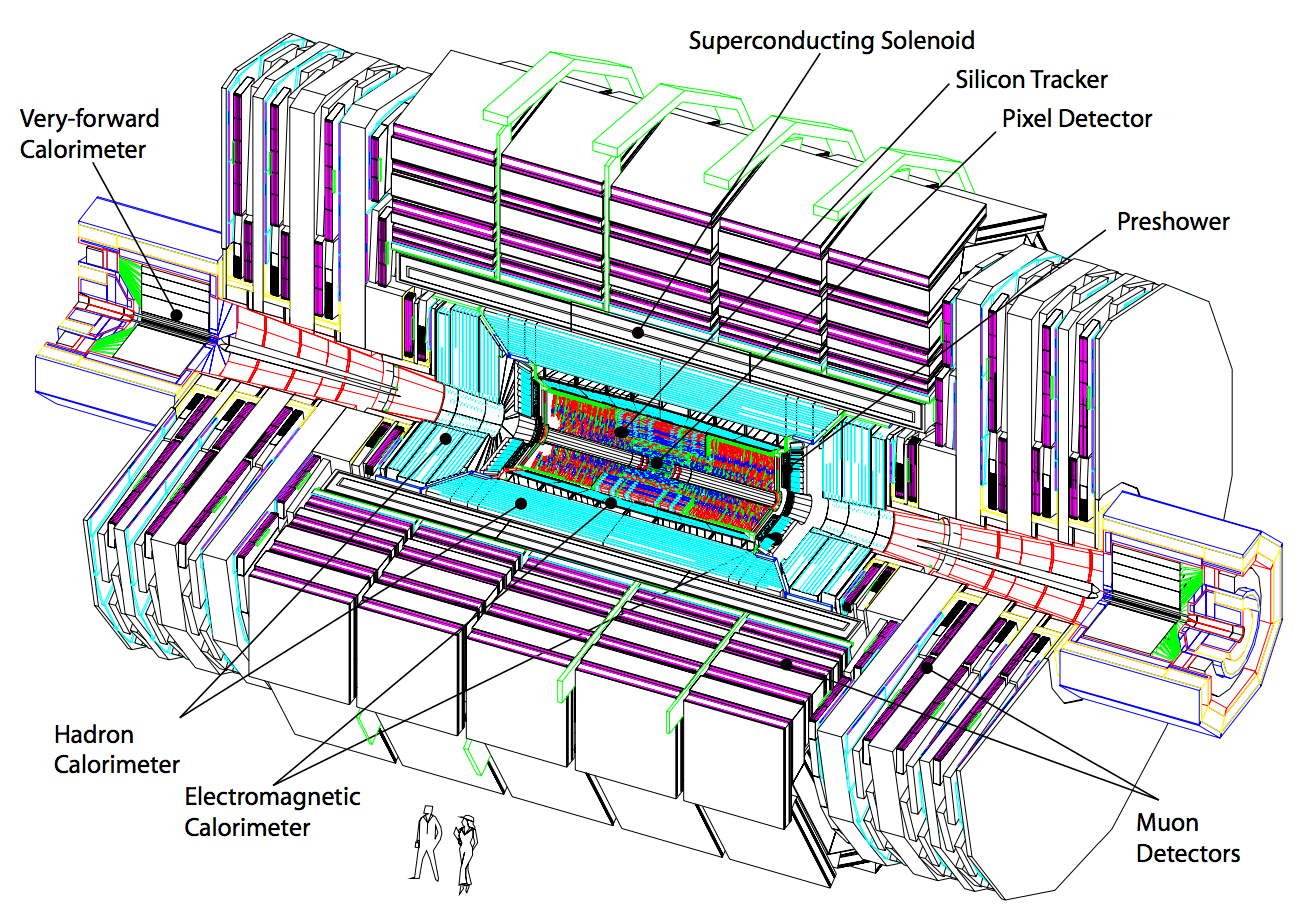
\includegraphics[width=\textwidth]{img/I-3-cms/cms.png}
      \caption{Schematic representation of the Compact Muon Solenoid detector installed at LHC \cite{1748-0221-3-08-S08004}.}
      \label{fig:I-3-cms-global-view}
    \end{figure}

    These requirements are met through the subdivision of CMS in various detection systems each specialised in the reconstruction of a given type of particles. The overall layout of CMS, which is shown in Figure \ref{fig:I-3-cms-global-view}, is divided into the barrel and the two endcaps, regions where the detectors are respectivly placed in parrallel and perpendicularly to the beam pipe. At the center of the detector, closest to the interaction point, lies the inner tracking system. Composed of 3 layers of silicon pixels and 10 layers of silicon strips detectors, it is designed to detect the passage of any charged particle with a high precision. Surrounding the tracking system are the electromagnetic and hadronic calorimeters which respectivly measure the energy of electrons and photons, and hadrons. These detectors are placed inside a superconducting solenoid magnet which produces a strong 3.8 T field that bends charged particles and allows for precise momentum measurments. Outside of the magnet, three different technologies of muon detectors are placed on large iron yokes.


  \section{The Inner Tracking System}

  \section{The Electromagnetic Calorimeter}

  \section{The Hadronic Calorimeter}

  \section{The Superconducting Magnet}

    \begin{figure}[h!]
      \centering
      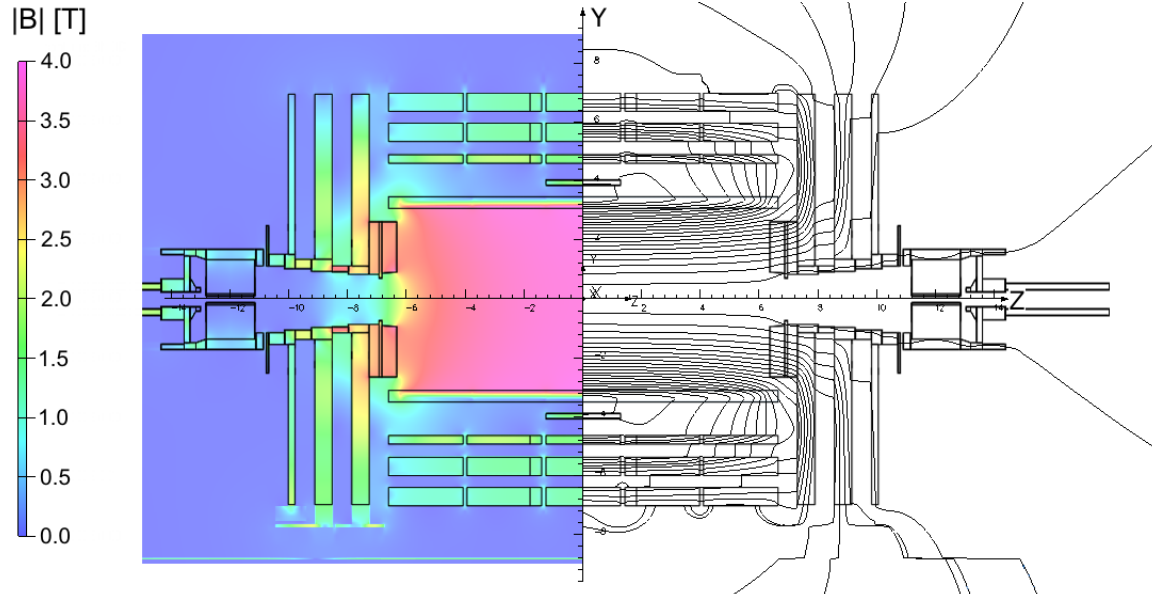
\includegraphics[width=\textwidth]{img/I-3-cms/magnet.png}
      \caption{??? \cite{Chatrchyan:2009si}.}
      \label{fig:I-3-cms-magnet}
    \end{figure}

  \section{The Muon System}

    \begin{figure}[h!]
      \centering
      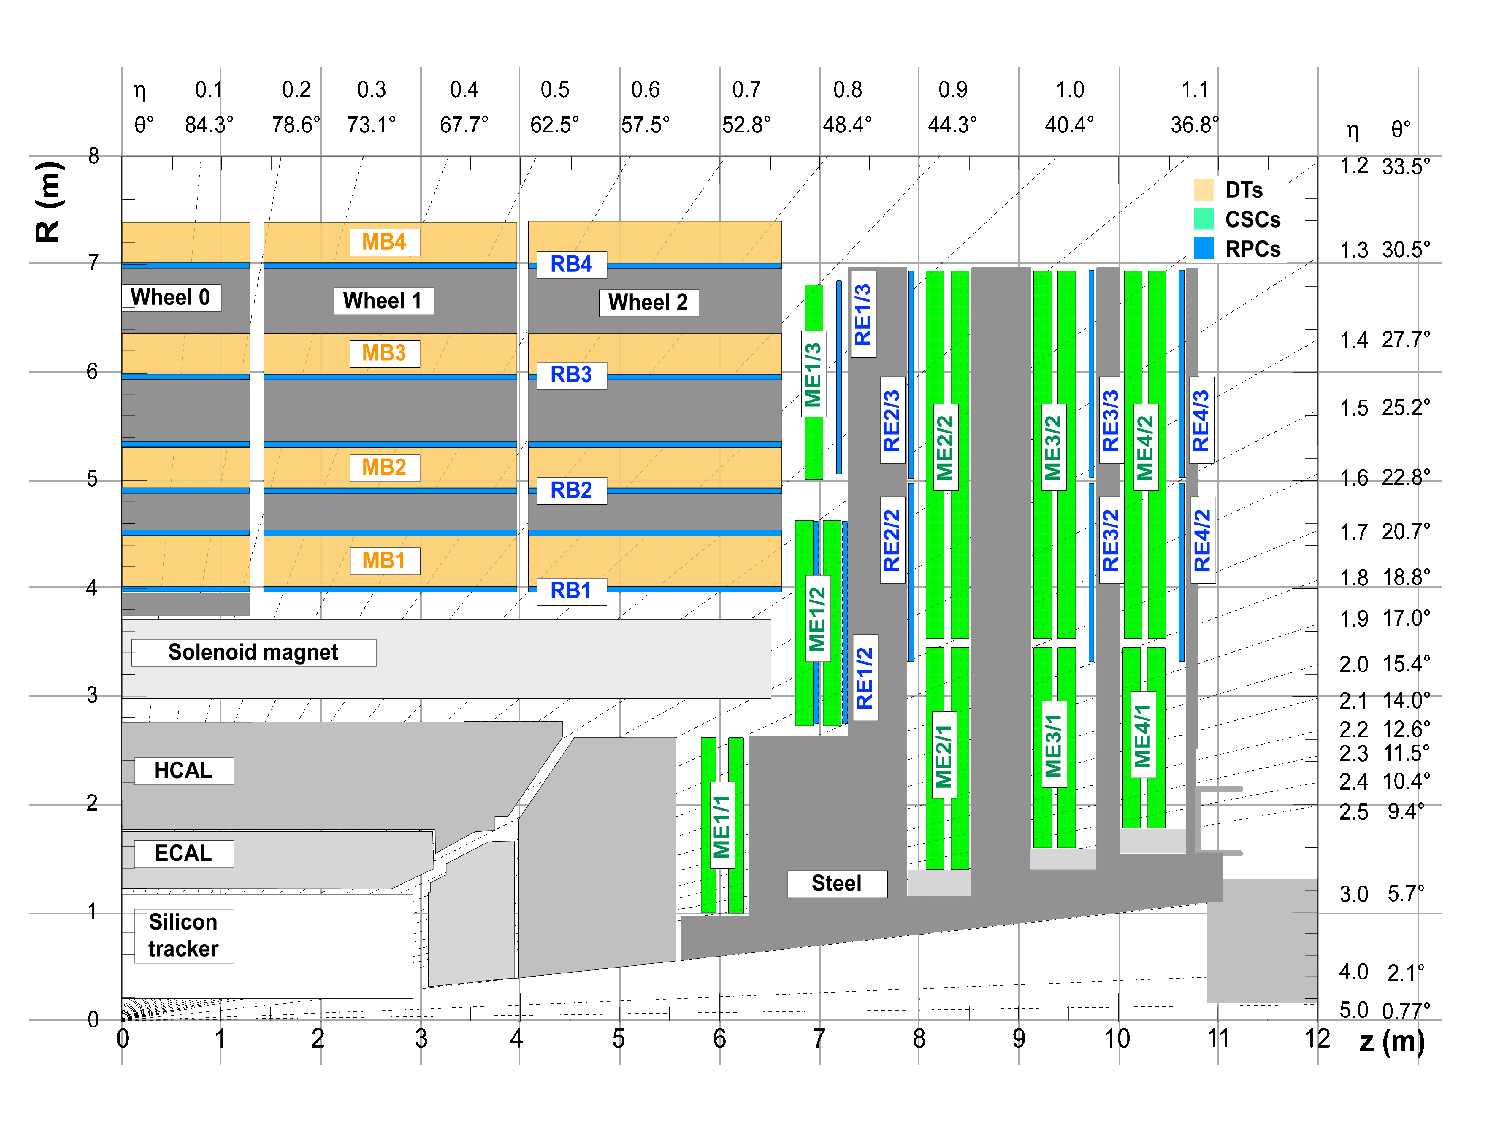
\includegraphics[width=\textwidth]{img/I-3-cms/quadrant-postls1.pdf}
      \caption{??? \cite{1748-0221-3-08-S08004}.}
      \label{fig:I-3-cms-quadrant}
    \end{figure}

    \begin{figure}[h!]
      \centering
      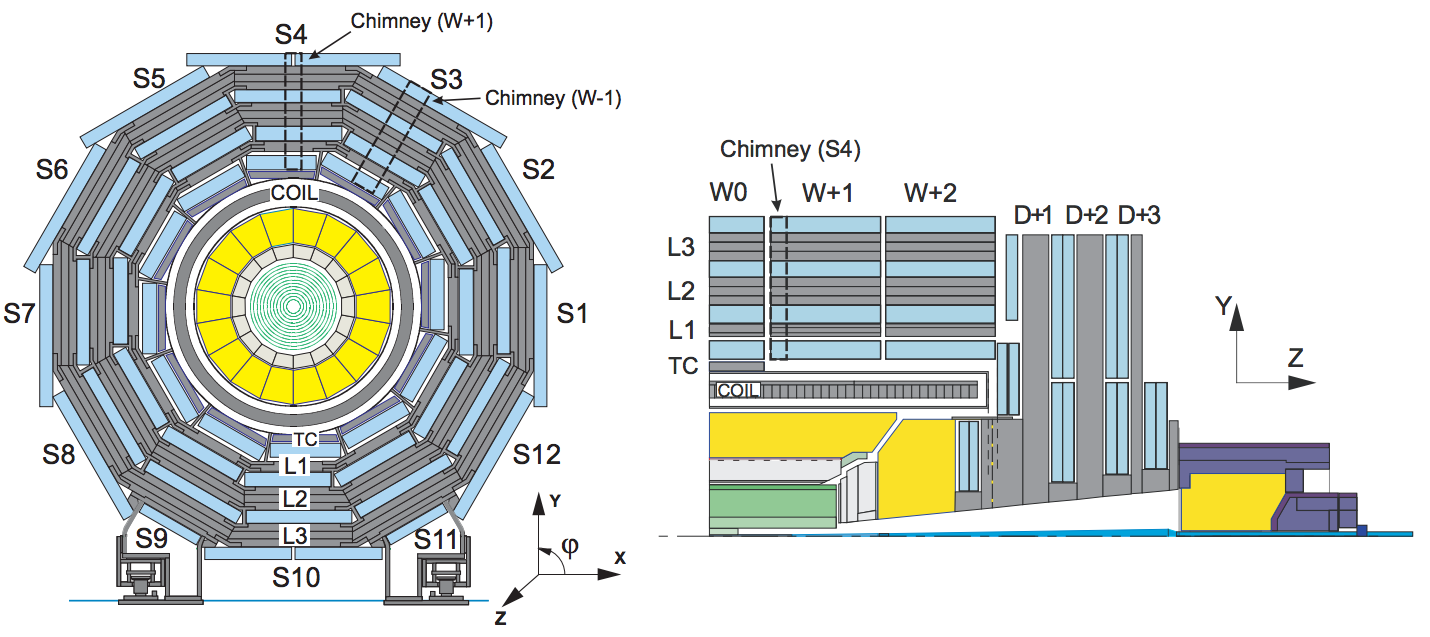
\includegraphics[width=\textwidth]{img/I-3-cms/muon-numbering.png}
      \caption{??? \cite{Chatrchyan:2009si}.}
      \label{fig:I-3-cms-muon-numbering}
    \end{figure}
























\newcommand{\GeVc}{GeV c$ ^{-1} $}
\newcommand{\um}{$ \mu $m}
\newcommand{\us}{$ \mu $s}
\newcommand{\pT}{$ p_T $}
\newcommand{\pZ}{$ p_Z $}
\newcommand{\axis}[1]{#1}

		The \emph{Compact Muon Solenoid} (CMS) \Cite{CMS_at_LHC} is, along with ATLAS, ALICE, and LHCb, one of the four main experiments recording the LHC beam collisions. Its structure and components are depicted in Figure \ref{fig:lhc_and_cms__cms_global_view}. As represented, it is composed of five main parts: the \emph{silicon tracker} (TK) in blue, the \emph{electromagnetic calorimeter} (ECAL) in green-blue, the \emph{hadronic calorimeter} (HCAL) in orange, the \emph{magnet} in purple, and the \emph{muon chambers} in white. \\

		\begin{figure}[h!]
			\centering
			% 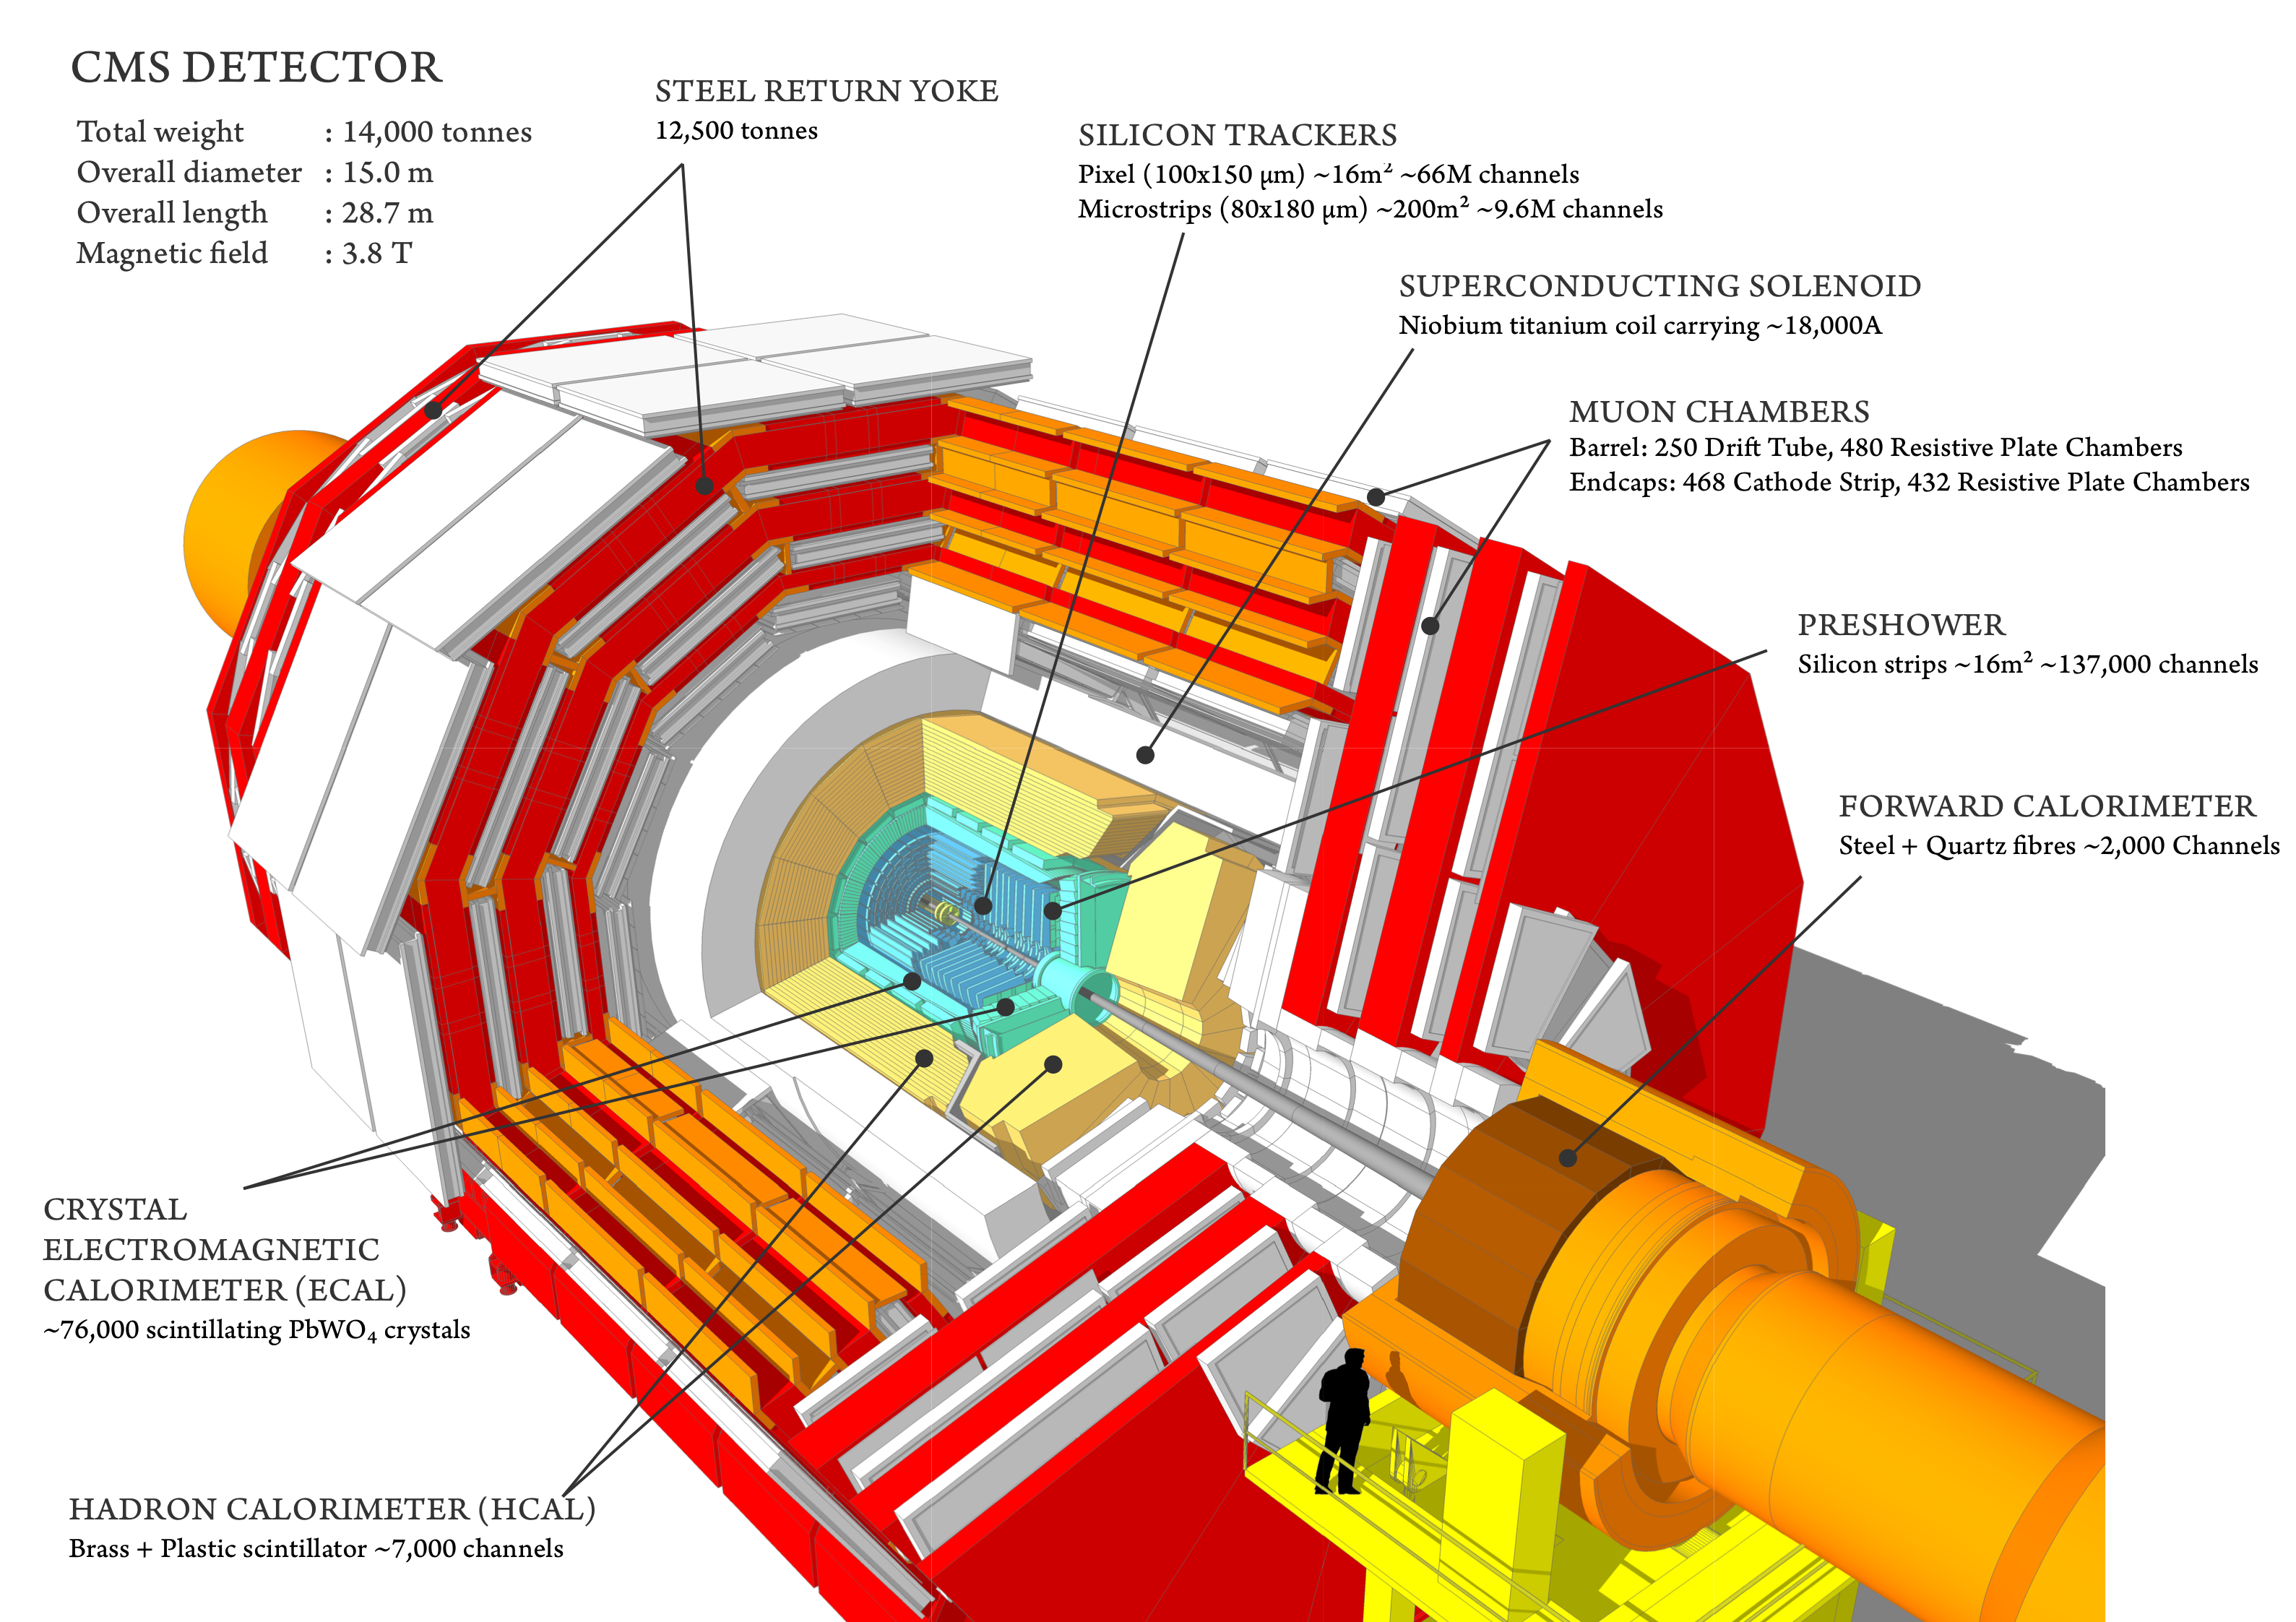
\includegraphics[width = 16.5cm]{2_LHC_CMS/img/cms_global_view.png}
			\caption{Representation of CMS and its different parts: the silicon tracker (blue), the electromagnetic calorimeter (green-blue), the hadronic calorimeter (orange), the magnet (purple), and the muon chambers (white) \Cite{Fig:cms-detector-design}.}
			\label{fig:lhc_and_cms__cms_global_view}
		\end{figure}

		CMS is divided into two regions: the barrel where the detectors are laid out cylindrically around the beam, and the endcaps where the detectors are placed perpendicularly to the beam. Although CMS has the ability to detect a wide range of interaction channels, it is characterized by its effective trigger system for muons and its strong magnetic field, which gave its name to the detector.

		\subsection{Appropriate Coordinates}
			\label{sec:lhc_and_cms__appropriated_coordinates}

			As CMS is of the cylindrical type, appropriate coordinates are defined to track particles. The Cartesian coordinates \axis{X}, \axis{Y}, and \axis{Z} are first set: \axis{X} points to the center of the accelerator, \axis{Y} to the surface, and \axis{Z} in the direction of the beam, as illustrated in Figure \ref{fig:lhc_and_cms__cms_coordinates}. The \axis{XY} plane is also referred to as the transverse plane. The problem with this set of coordinates is that the physics is not symmetrical under these, which would be a beneficial feature. Therefore, the rapidity $ y $, a Lorentz invariant over which the particles in the final state are equally distributed, is used. The rapidity is defined as
			\begin{equation}
				y = \frac{1}{2} \ln \left( \frac{E + p_Z}{E - p_Z} \right) \ ,
			\end{equation}
			which for highly relativistic particles can be approximated by the pseudo-rapidity
			\begin{equation}
				\eta = - \ln \left[ \tan \left( \frac{\theta}{2} \right) \right] \ ,
			\end{equation}
			where $ \theta $ is the polar angle (angle between the particle and the \axis{Z} axis). The other coordinates are the azimuth $ \phi $ (angle in the \axis{XY} plane), and the distance to the beam in the transverse plane $ R $ for tracks the barrel, and the \axis{Z} coordinate for tracks the endcaps. \\

			\begin{figure}[h!]
				\centering
				% 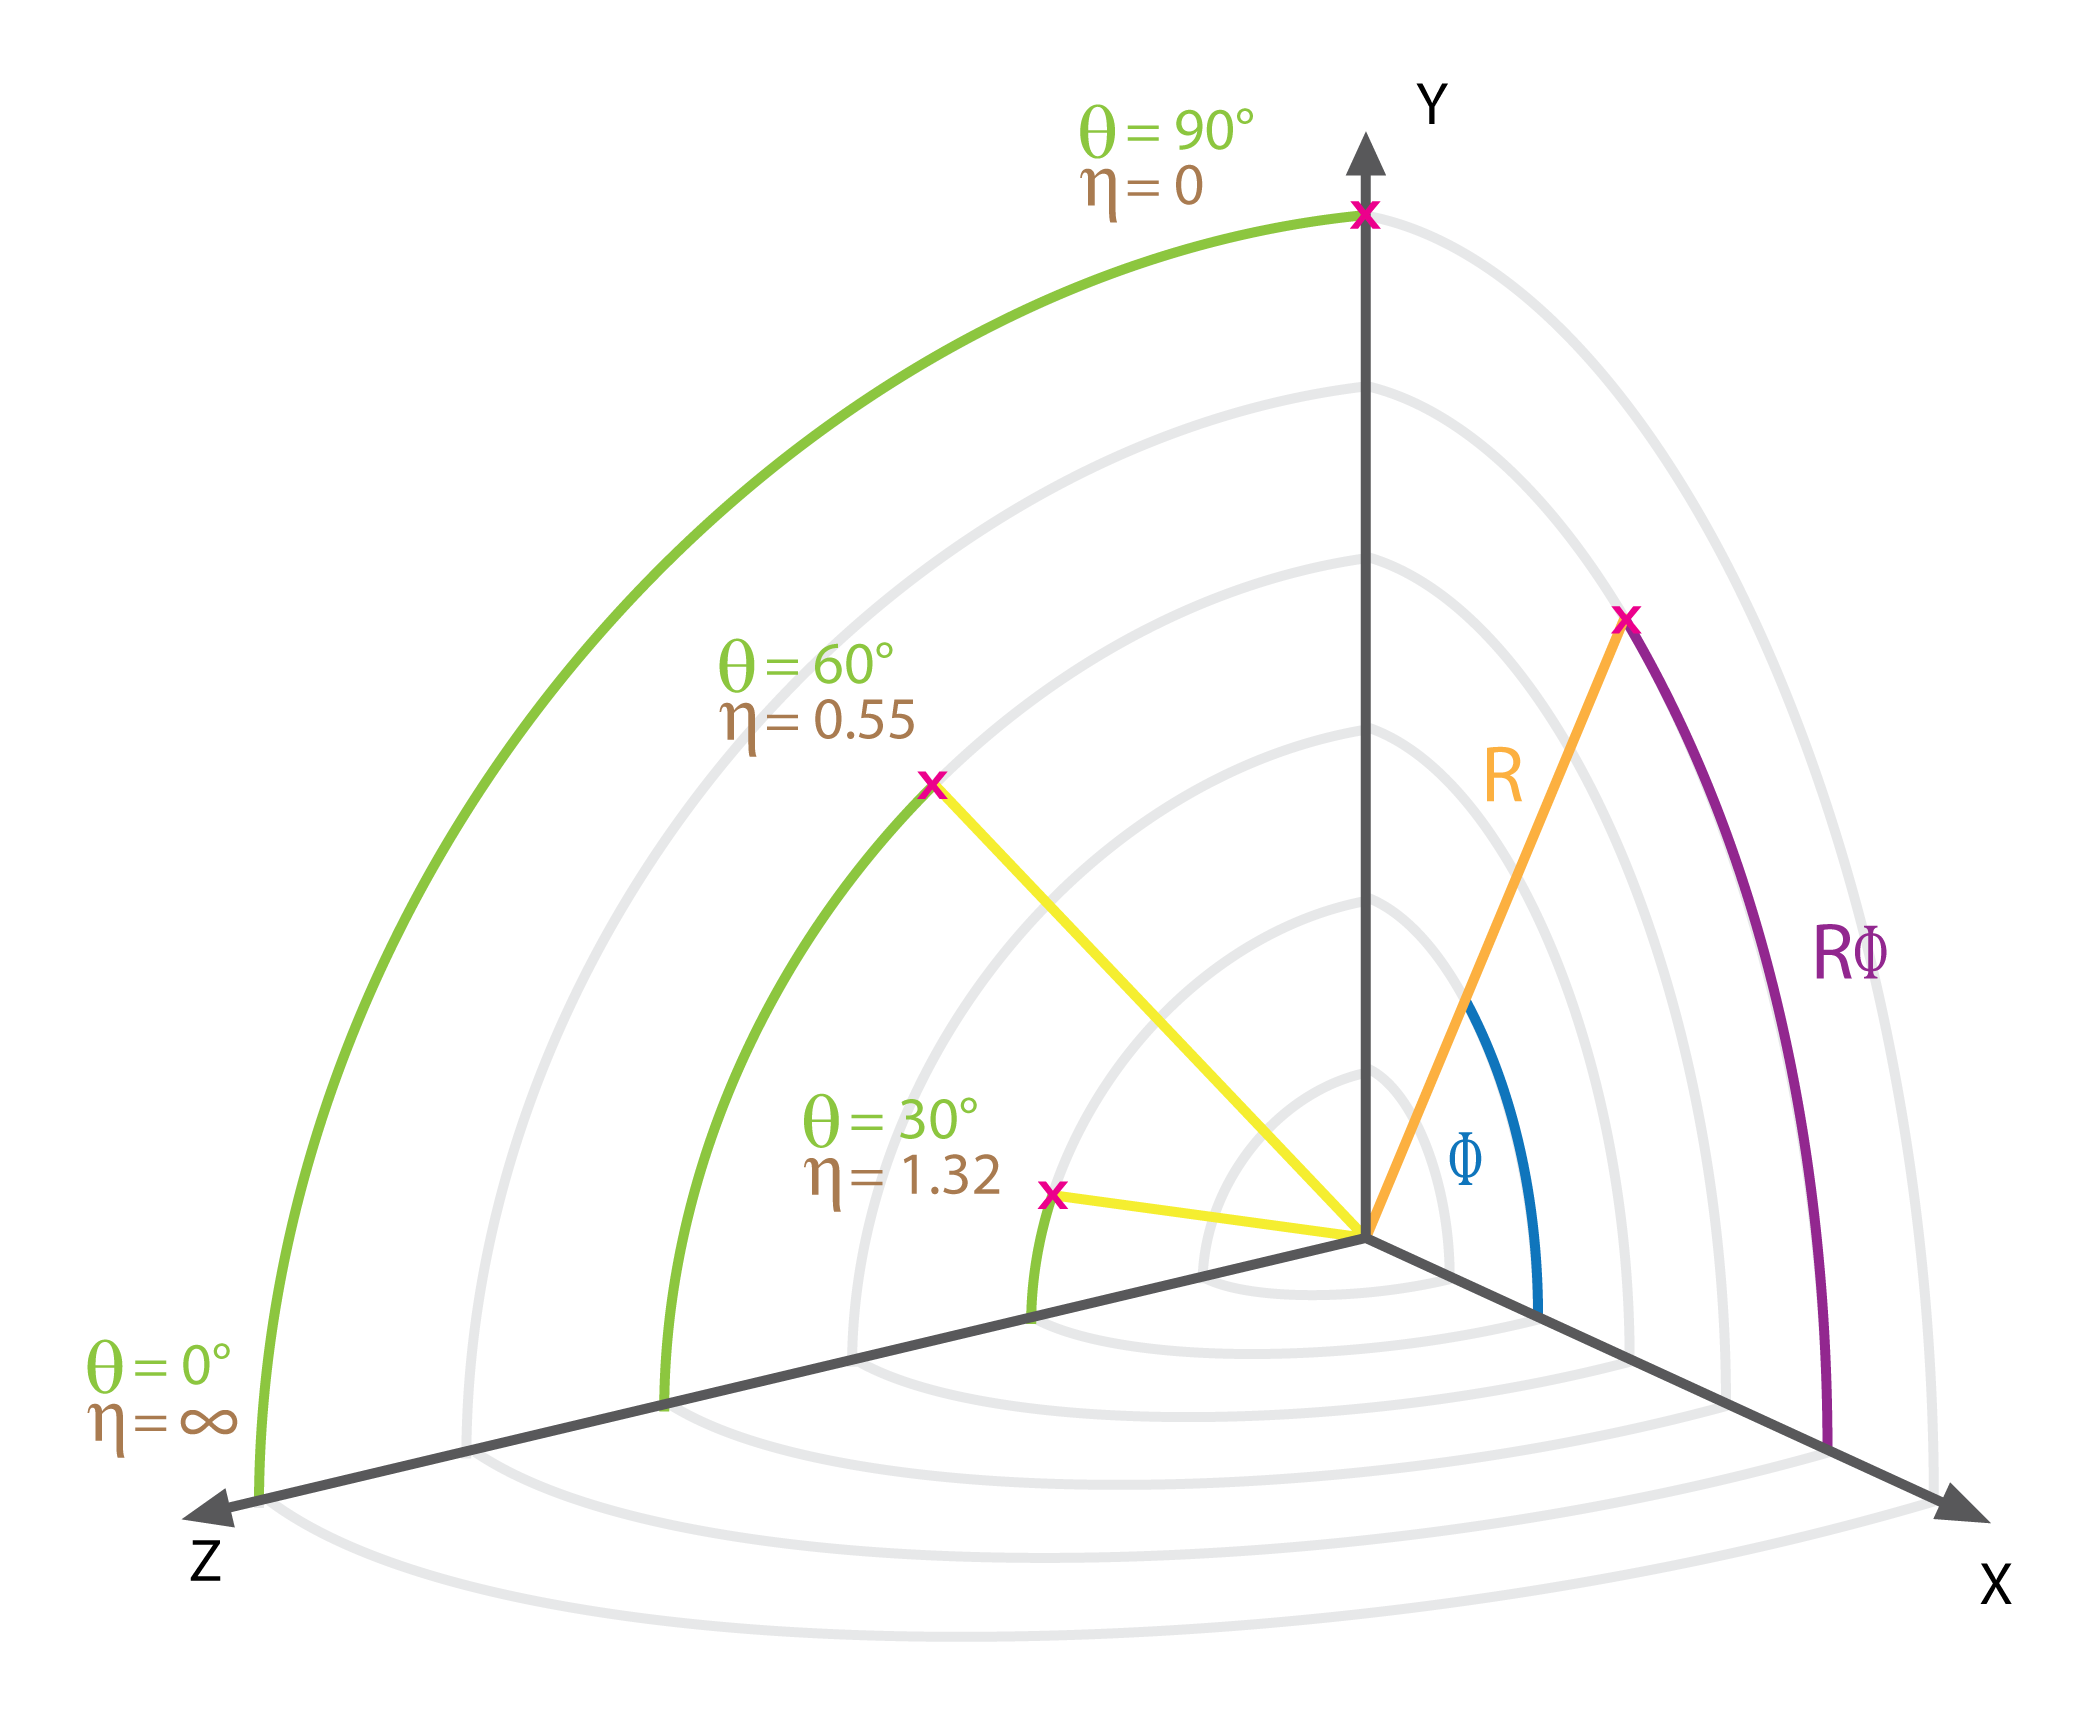
\includegraphics[width = 11cm]{2_LHC_CMS/img/cms_coordinates.png}
				\caption{Pseudo-rapidity $ \eta $ and azimuthal angle $ \phi $ used to track particles inside CMS.}
				\label{fig:lhc_and_cms__cms_coordinates}
			\end{figure}

			As previously stated, the particles in the final state are equally distributed over $ \eta $. This means that the particles fluxes are lower in the barrel than in the endcaps. This impacts the detectors' geometry.

		\subsection{Silicon Tracker}
		\label{sec:lhc_and_cms__tracker}

			The silicon tracker is the detector closest to the IP. It is composed of two different types of semiconductor detectors: \emph{silicon pixels} and \emph{silicon strips}. These detectors have an excellent spatial resolution (down to 25 \um{}) which yields excellent momentum reconstruction capabilities (resolution of the order of 1\% at low transverse momenta). The disposition of the different technologies is represented in Figure \ref{fig:lhc_and_cms__cms_tracker}. The silicon pixels are represented in blue, while TIB, TID, TOB, and TEC refer to different regions of the silicon strip detector. \\

			\begin{figure}[h!]
				\centering
				% 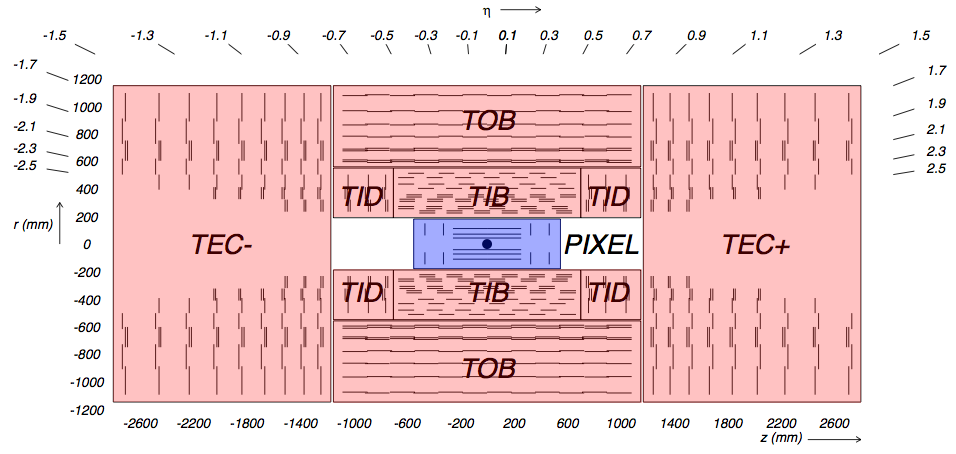
\includegraphics[width = 13cm]{2_LHC_CMS/img/cms_tracker_view.png}
				\caption{Disposition of the different detectors in the silicon tracker. PIXEL (blue) refers to silicon pixel detectors while TIB, TID, TOB and TEC (red) all refer to silicon strip detectors \Cite{CMS_at_LHC}.}
				\label{fig:lhc_and_cms__cms_tracker}
			\end{figure}

			Semiconductor detectors are made out of two pieces of silicon, one negatively doped containing more unbounded electrons, and one positively doped containing more unbounded holes (absence of electrons), put together to form a n-p junction. At the interface, the electrons and the holes diffuse in the opposite region and recombine with the particles of opposite charge, creating an unbalance in charge: the n region and p region close to the junction become, respectively, positively and negatively charged. From this, an electric field is formed which slows the diffusion down until the system reaches equilibrium. When a charged particle passes through this region and losses energy, electrons switch from non-conductive to conductive bands creating electrons/holes pairs. Under the action of the electric field, they migrate towards the n or p regions and form the signal on the readout electronics. Unfortunately, the number of unbounded charges is still high compared to the formed signal and the active region is small. To increase the detection efficiency, a voltage difference is applied to the semiconductor further diffusing the electrons and holes through the junction. Typically, for a voltage difference of 100 V, the size of the active region is of the order of 300 \um{}.

			\subsubsection{Silicon Pixel Detectors}
			\label{sec:lhc_and_cms__silicon_pixel_detectors}

				The silicon pixels detectors, represented in Figure \ref{fig:lhc_and_cms__cms_pixel_detector}, are composed of small 100 \um{} x 150 \um{} rectangles of readout material disposed on a block of detection medium formed by a n-p region. The electrons are formed in that region and migrate towards the silicon pixels. The challenge arising is that each pixel needs its own readout electronics which takes a significant amount of space and requires output cables. These cables prevent the placing of detectors which creates dead-zones. Physicists and engineers must find the right balance between the number of pixels (granularity), the size of the electronic, and the detectors' resolution. \\

				\begin{figure}[h!]
					\centering
					% 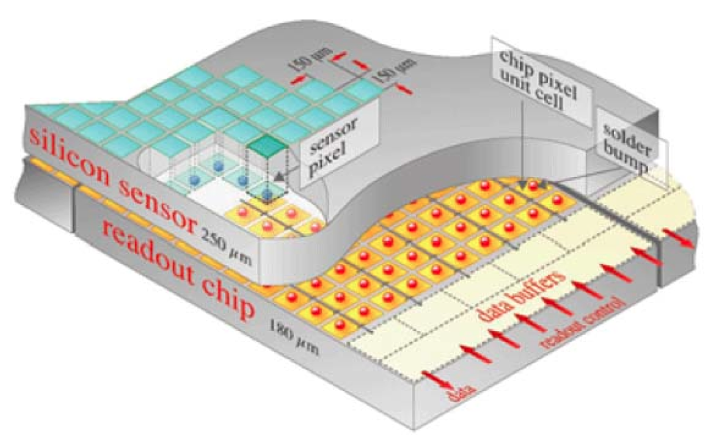
\includegraphics[width = 8cm]{2_LHC_CMS/img/cms_tracker_pixel.png}
					\caption{Disposition of the readout pixels (orange and red) on the same detection block (gray) inside a silicon pixel detector \Cite{CMS_Tracker_Construction}.}
					\label{fig:lhc_and_cms__cms_pixel_detector}
				\end{figure}

				Nevertheless, the pixel detectors are the most precise tracking technology in CMS with a spatial resolution of 15 to 20 \um{}. This value is smaller than the size of the pixels because of \emph{charge sharing}. All the pixels sharing the same detection block also share the energy deposited by a particle. By reading the total deposited charge on each of the pixels, we can find the \emph{Center of Gravity} (COG). The COG method is based on the assumption that there exists a linear relation between the induced pulse's height on a pixel and the distance between its center and the particle's hit, so that each pixel is assigned a weight proportional to the deposited charge. The reconstructed coordinate $ \mathbf{x}_{COG} $ of the cluster is then given by
				\begin{equation}
					\mathbf{x}_{COG} = \frac{\sum_i \mathbf{x}_i q_i}{\sum_i q_i} \ ,
					\label{eq:lhc_and_cms__charge_sharing}
				\end{equation}
				where $ q_i $ is the individual pixel signal in the cluster, and $ \mathbf{x}_i $ is the positions of the pixel in the defined coordinate system. The same technique can be applied to other detectors as long as the charge is read out analogically and not digitally\footnote{One can consider using the same method with digital readouts but will not be able to achieve the same resolutions.}.

			\subsubsection{Silicon Strip Detectors}
			\label{sec:lhc_and_cms__silicon_strip_detectors}

				The most outer layers of the tracker cannot have a granularity as high as the pixel detectors, for both financial and technical reasons. The amount of data that would have to be read out is considerable, and the technology to do so is not yet available. A way to reduce the granularity of the detectors is to measure only one coordinate by using silicon strips instead of pixels. The strips are separated by 80 to 122 \um{} which gives a resolution between 23 \um{} and 53 \um{} in the direction perpendicular to the strips. Unfortunately, as expected, there is a larger error on the other coordinate (along the strip) corresponding to the size of the detection cell. To improve global precision, some of the cells have two strip detectors placed with a small stereo angle, typically 100 mrad, allowing them to measure both coordinates. However, this set up generates \emph{ghosts} because of the ambiguity created when more than one particle hits the detector at the same time.

			\subsubsection{System Performances}
			\label{sec:lhc_and_cms__tracker_system_performances}

				Due to the magnetic field generated by the solenoid, the trajectories charged particles are bent inside the tracker. The relation between the bending radius of the track $ R $ , the transverse momentum $ p_T $, and the intensity of the magnetic field $ B $ is
				\begin{equation}
					R[\mbox{m}] = \frac{p_T[\mbox{GeV c}^{-1}]}{0.3 B[\mbox{T}]} \ .
					\label{eq:lhc_and_cms__radius_to_momentum_relation}
				\end{equation}
				By measuring the bending radius of the track and inverting the previous relation, the transverse momentum of the particles can be obtained. Tracks created by high energy particles will be straighter than those left by low energy particles and therefore more difficult to reconstruct. \\

				As previously stated, the tracker offers an excellent resolution on the position of the particles and therefore gives precise measurements of the particles' momentum. Figure \ref{fig:lhc_and_cms__cms_tracker_performances} shows the resolution on the transverse momentum \pT{} (left) and detection efficiency (right) of the tracker as a function of the pseudo-rapidity $ \eta $ for muons of transverse momenta \pT{} of 1, 10, and 100 \GeVc{}. The resolution is less than 1\% for muons of 1 and 10 \GeVc{} in the barrel ($ \eta $ < 1) and quickly rises in the most forward region. The same effect is observed for the detection efficiency which is close to 100\% in the barrel but significantly diminishes at higher pseudo-rapidities. Precision decreases in the most forward region where the strip pitch is greater and more material is present, causing more scatterings.

				\begin{figure}[h!]
					\centering
					% 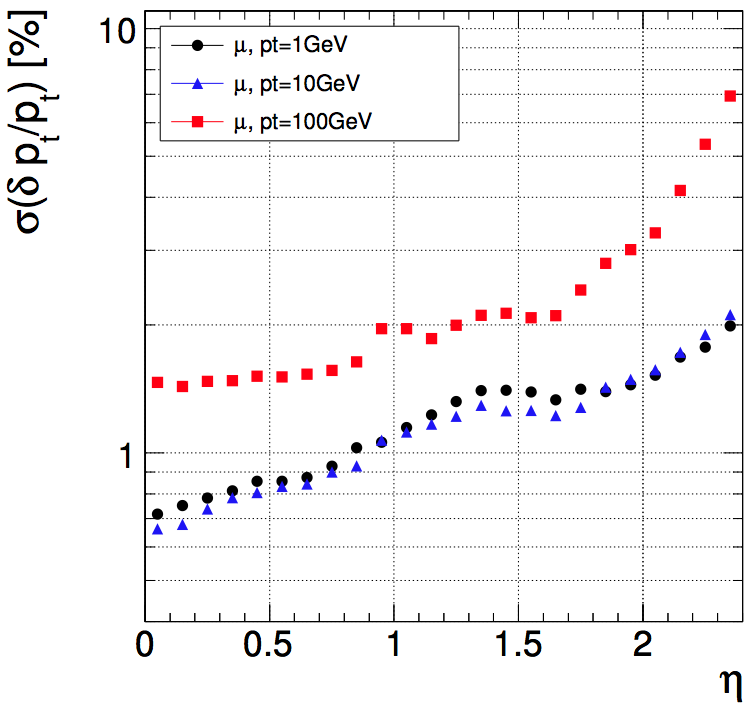
\includegraphics[width = 6.3cm]{2_LHC_CMS/img/cms_tracker_resolution.png}
					% 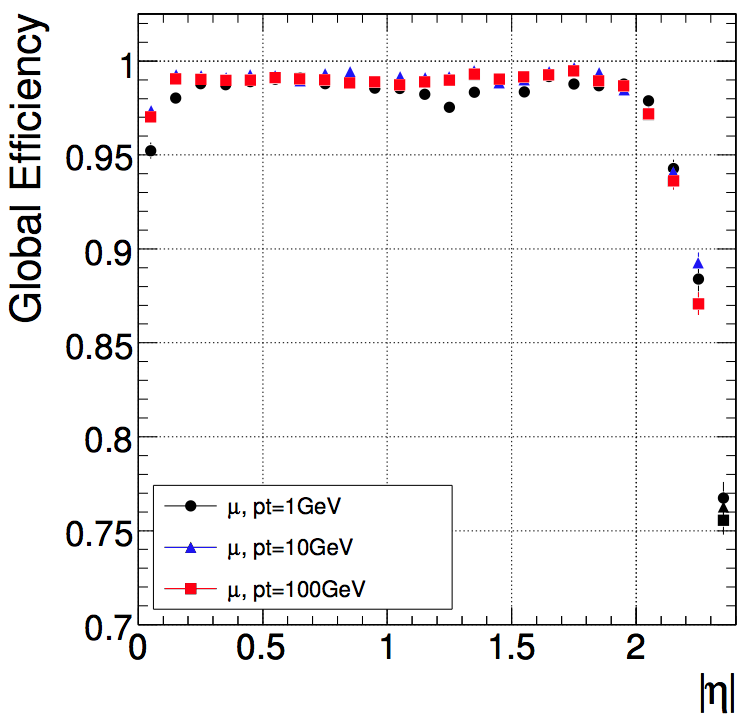
\includegraphics[width = 6.3cm]{2_LHC_CMS/img/cms_tracker_efficiency.png}
					\caption{Resolution on the transverse momentum \pT{} (left) and detection efficiency (right) of the tracker as a function of the pseudo-rapidity $ \eta $ for muons of transverse momenta \pT{} of 1, 10, and 100 \GeVc{} \Cite{CMS_at_LHC}.}
					\label{fig:lhc_and_cms__cms_tracker_performances}
				\end{figure}

		\subsection{Calorimeters}
		\label{sec:lhc_and_cms__calorimeters}

			Calorimeters are devices that absorb the full kinetic energy of a particle by creating particle cascades, and provide a signal that is proportional to that deposited energy. \\

			Two types of calorimeters are present in CMS: the electromagnetic to detect electrons and photons, and the hadronic to detect hadrons. Each of them corresponding to two of the elementary interactions through which particles can interact with the medium: electromagnetic interaction and strong interaction. \\

			The parameters characterizing particles showers are the radiation length $ \lambda_R $, and the Molière radius $ R_M $ for the electromagnetic calorimeter, and the absorption length $ \lambda_a $ and the interaction length $ \lambda_I $ for the hadronic calorimeter, all depending upon the atomic properties of the material.
			\begin{enumerate}
				\item[] $ \lambda_R $ is the distance that an electron or photon has to travel inside the calorimeter to, respectively, emit a photon or create an electron/positron pair.
				\item[] $ R_M $ gives the radius of the cylinder in which 90\% of the electromagnetic shower is contained.
				\item[] $ \lambda_a $ is the average distance that a hadron has to travel before undergoing an inelastic interaction with the medium.
				\item[] $ \lambda_I $ yields the distance after which a hadron will have scattered inelastically and also gives the radius of the cylinder in which 95\% of the hadronic shower is contained.
			\end{enumerate}
			Those parameters result in the spatial extension of the cascades giving an idea of the granularity needed to correctly distinguish showers. Because the interaction length $ \lambda_I $ of hadrons is much larger than the radiation length $ \lambda_R $ of electrons and photons, the ECAL is placed first. This also implies that hadrons can pass through the ECAL without interacting, or at least not significantly, even if it is multiple $ \lambda_R $ long. \\

			The energy resolution of calorimeters depends upon the number of particles in the cascade hence the energy of the particle
			\begin{equation}
				\left( \frac{\sigma_E}{E} \right)^2 = \left( \frac{a}{\sqrt{E}} \right)^2 + \left( b \right)^2 + \left( \frac{c}{E} \right)^2 \ ,
			\end{equation}
			where $ a $ is the stochastic term depending upon the development of the shower and the detector's response, $ b $ is the constant term determined by the calibration and the uniformity of the crystal, and $ c $ is the noise term from the electronics. Unlike the tracker, the calorimeters' resolution increases with the energy, offering the best resolution at high energies.

			\subsubsection{Electromagnetic Calorimeter}
			\label{sec:lhc_and_cms__electromagnetic_calorimeter}

				The two main processes allowing the detection of electrons and photons are respectively Brëmsstrahlung and pair creation. These occur as long as the resulting particles (electrons and photons) have enough energy to repeat the process, creating an electromagnetic cascade inside the material. The size of the cascade hence the number of photons emitted by the scintillator is proportional to the energy of the incident particle. Muons do not significantly interact with the ECAL because the radiative processes are greatly suppressed. Indeed, Brëmsstrahlung is proportional to m$ ^{-2} $ (inverse-squared mass) and is therefore only significant for electrons. \\

				\begin{figure}[h!]
					\centering
					% 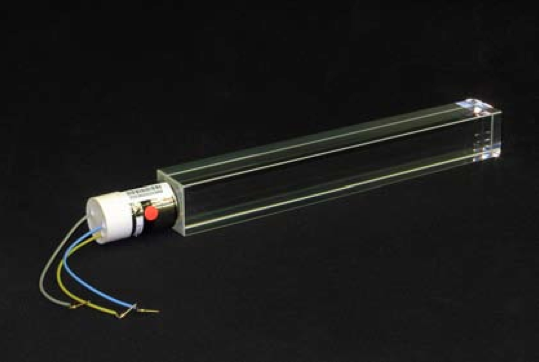
\includegraphics[height = 4cm]{2_LHC_CMS/img/cms_ecal_crystal.png}
					% 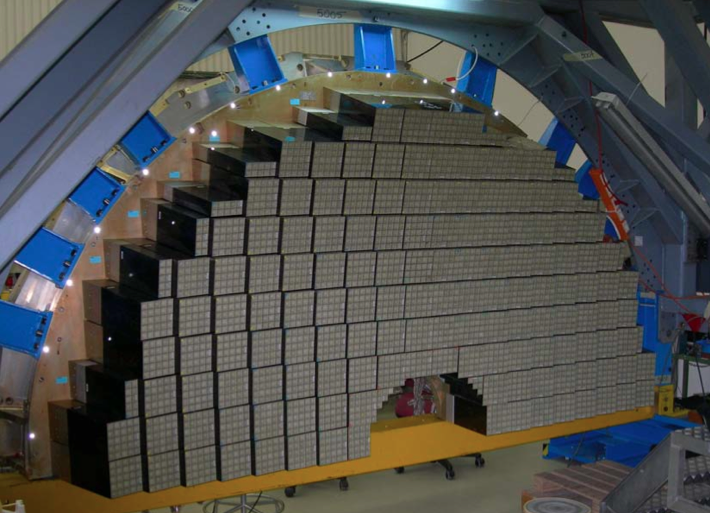
\includegraphics[height = 4cm]{2_LHC_CMS/img/cms_ecal_endcap.png}
					\caption{Picture of a PbWO$ _4 $ crystal (left) used in the ECAL with its photomultiplier, and of the endcap ECAL (right) showing the crates in which the crystals are placed \Cite{CMS_at_LHC}.}
					\label{fig:lhc_and_cms__cms_ecal_view}
				\end{figure}

				In CMS, the ECAL is composed of PbWO$ _4 $ crystals, acting both as interaction media and as scintillators, attached to photomultipliers to amplify the relatively small amount of photons they emit. The crystals measure 2.2 cm x 2.2 cm, which is equivalent to one Molière radius $ R_M $, by 23 cm, which corresponds to several radiation lengths $ X_0 $. Figure \ref{fig:lhc_and_cms__cms_ecal_view} shows one of these crystals (left), the crates that hold them, and their disposition in the endcap (right). The number of photons collected is proportional to the energy deposited in the calorimeter modulo a correction factor due to the aging of the material. The ambient radiation causes the crystals to become opaque and release less photons which in turn implies a constant need for recalibration of the detectors.

			\subsubsection{Hadronic Calorimeter}
			\label{sec:lhc_and_cms__hadronic_calorimeter}

				Where the ECAL relies on radiative processes to detect particles, the HCAL uses strong interactions between the hadrons and the material to create hadronic cascades. These are much longer than electromagnetic showers, requiring longer detectors. The most created particles are pions as they are the lightest hadrons. This induces an electromagnetic component as the $ \pi^0 $ principal decay channel is $ \pi^0 \rightarrow \gamma \gamma $. This creates a problem, as the response of the material can be different for the hadronic and electromagnetic component. \\

				Figures \ref{fig:lhc_and_cms__cms_hcal_view} are a picture of a section of the barrel HCAL representing the absorber (golden plates) with the scintillator in between and of the installation of the barrel HCAL in CMS. The HCAL is composed of an alternation of 16 layers of absorbers, made out of 40 to 70 mm thick steel plates and 50 to 56 mm thick 70\% Cu and 30\% Zn alloy plates, and 3.7 to 9 mm thick plastic scintillators. When particles hit the detectors perpendicularly, they have to travel through 79 cm of matter equivalent to 5.82 interaction lengths $ \lambda_I $. The barrel HCAL is divided into 72 segments in $ \phi $ and 16 $ \eta $ sectors while the endcap HCAL has 36 and 72 $ \phi $ segments for the inners and outers rings respectively, and 14 $ \eta $ sectors.

				\begin{figure}[h!]
					\centering
					% 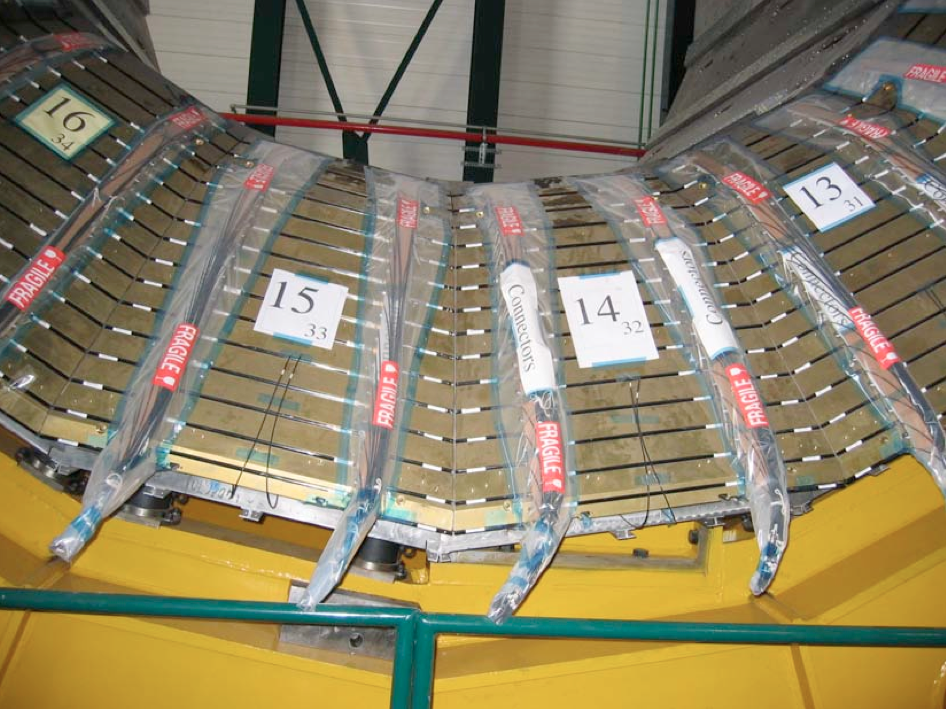
\includegraphics[height = 5cm]{2_LHC_CMS/img/cms_hcal.png}
					% 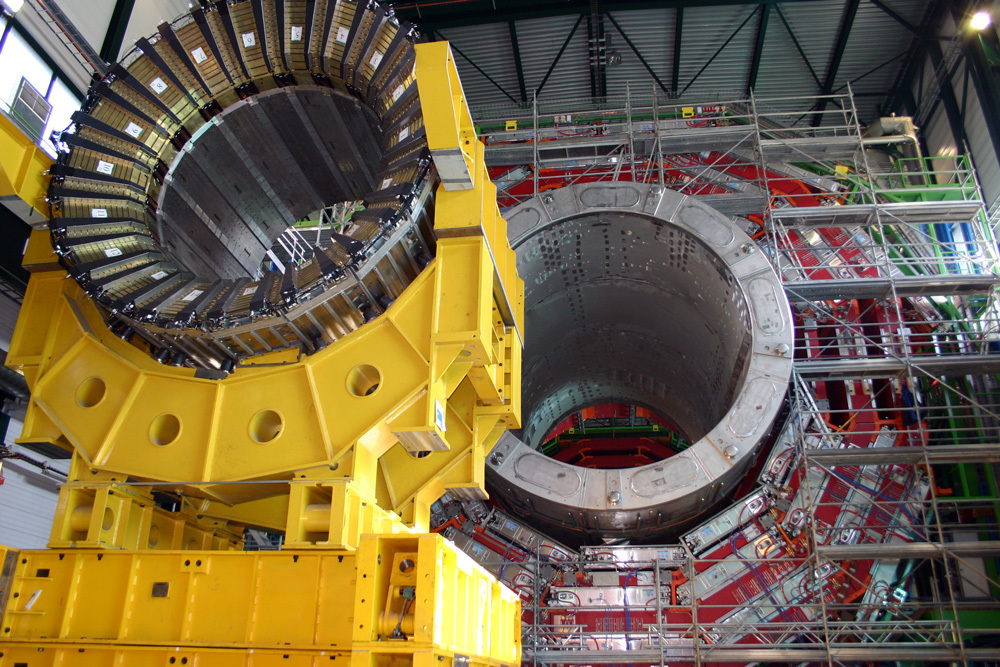
\includegraphics[height = 5cm]{2_LHC_CMS/img/cms_hcal_install.jpg}
					\caption{Picture of the barrel HCAL composed of several dense absorber (golden plates) and smaller scintillators placed in between (left) \Cite{CMS_at_LHC}, and installation in CMS of the barrel HCAL (right) \Cite{CMS_HCAL_Install}}
					\label{fig:lhc_and_cms__cms_hcal_view}
				\end{figure}

			\subsubsection{System Performances}
			\label{sec:lhc_and_cms__calorimeters_system_performances}

				The CMS ECAL's energy resolution is \Cite{CMS_Performances}
				\begin{equation}
					\left( \frac{\sigma_E}{E} \right)^2 = \left( \frac{2.8\%}{\sqrt{E}} \right)^2 + \left( 0.30\% \right)^2 + \left( \frac{0.12}{E} \right)^2 \ ,
				\end{equation}
				where $ E $ is given in GeV. The CMS HCAL's energy resolution is
				\begin{equation}
					\left( \frac{\sigma_E}{E} \right)^2 = \left( \frac{120\%}{\sqrt{E}} \right)^2 + \left( 6.9\% \right)^2 \ .
				\end{equation}

		\subsection{Solenoid}
		\label{sec:lhc_and_cms__solenoid}

			The intense magnetic field of CMS is created by cooling a solenoid down to 4.5 K, temperature at which the metal becomes supra-conductive, and by passing strong currents through it. The resulting field is uniform inside the solenoid but more complex outside, as shown in Figure \ref{fig:lhc_and_cms__cms_magnetic_field} which represents the measured magnetic field. The constant and strong field in which the tracker is placed allows it to measure the particles' transverse momentum with high-precision (resolution of less than 1\% in the tracker as seen in Figure \ref{fig:lhc_and_cms__cms_tracker_performances}). The intensity of the field is of 3.8 T inside the solenoid and typically 2 T outside the solenoid. \\

			\begin{figure}[h!]
				\centering
				% 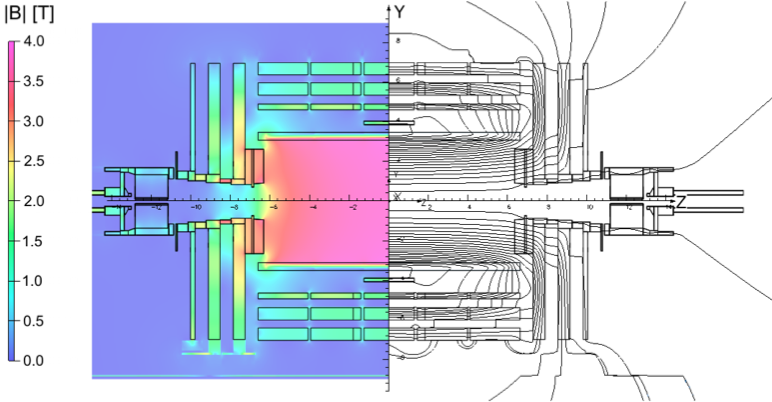
\includegraphics[width = 12cm]{2_LHC_CMS/img/cms_magnetic_field.png}
				\caption{Field map of the magnetic field of CMS measured using cosmic rays \Cite{CMS_B_Field}.}
				\label{fig:lhc_and_cms__cms_magnetic_field}
			\end{figure}

			Having the calorimeters inside the magnet improves the energy resolution as particles have less matter to travel through before reaching them, but increases the size of the solenoid. Due to the technical difficulty to build large magnets, the muon chambers are placed on the outside. This layout has the advantage to use the magnet as barrier for most particles escaping the calorimeters, ensuring that only muons will be detected by the muon system.

		\subsection{Muon Chambers}
		\label{sec:lhc_and_cms__muon_chambers}

			The muons system is composed of several types of gaseous detectors which physics and functioning are exposed in the next chapter. They are placed in the outer section of CMS because muons are the only detectable particles left at this stage as they do not or slightly interact with the calorimeters.
